\documentclass[tikz]{standalone}

\usepackage[latin1]{inputenc}
\usepackage{tikz}
\usetikzlibrary{decorations.markings}

% GNUPL
\begin{document}
\pagestyle{empty}


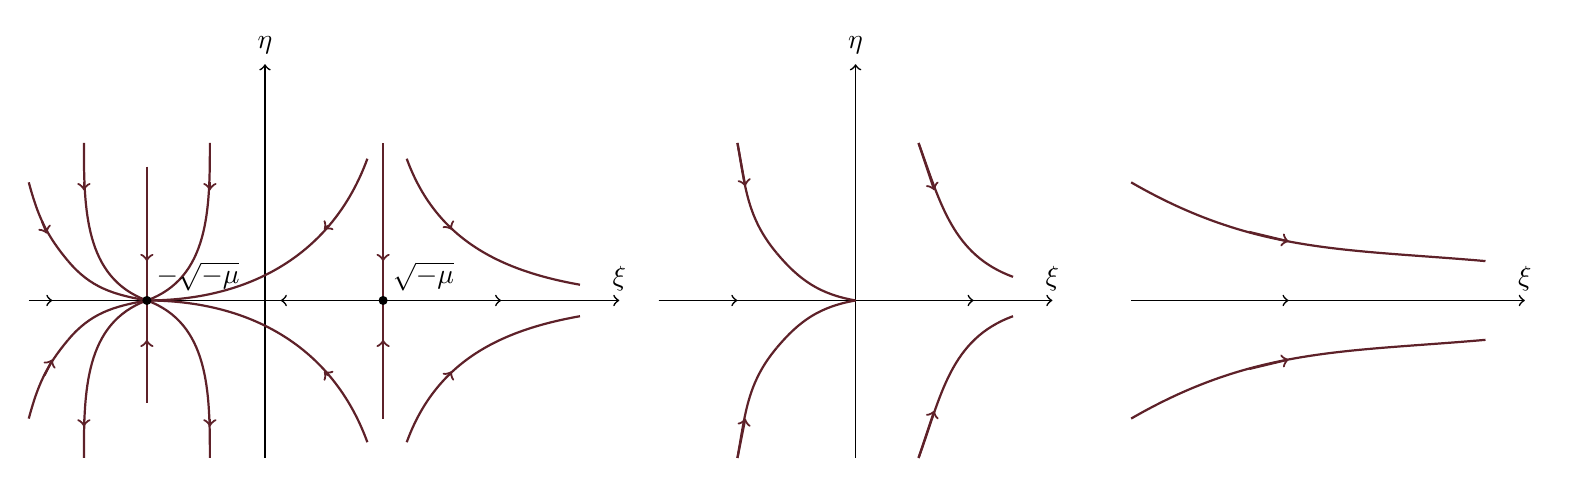
\begin{tikzpicture}
    %\mu<0
    \draw[semithick] [->] (0,3) -- (7.5,3) node[above] {$\xi$};
    \draw[semithick] [->] (0,3) -- (0.3,3);
    \draw[semithick] [->] (3.5,3) -- (3.2,3);
    \draw[semithick] [->] (5.8,3) -- (6,3);
	\draw[semithick] [->] (3,1) -- (3,6) node[above] {$\eta$};
	\draw [color={rgb,255:red,94; green,33; blue,41}, thick] (1.5,1.7) -- (1.5,3);
	\draw [color={rgb,255:red,94; green,33; blue,41}, thick] (1.5,4.7) -- (1.5,3);
	\draw [color={rgb,255:red,94; green,33; blue,41}, thick] [->] (1.5,2) -- (1.5,2.5);
	\draw [color={rgb,255:red,94; green,33; blue,41}, thick] [->] (1.5,4) -- (1.5,3.5);
    \draw [color={rgb,255:red,94; green,33; blue,41},thick] (0,1.5) to [out=75,in=-130] (0.5,2.5);
    \draw [color={rgb,255:red,94; green,33; blue,41}, thick] [->] (0.2,2.05) -- (0.3,2.25);
    \draw [color={rgb,255:red,94; green,33; blue,41},thick] (0.5,2.5) to [out=50,in=-170] (1.5,3);  
    \draw [color={rgb,255:red,94; green,33; blue,41},thick] (0,4.5) to [out=-75,in=130] (0.5,3.5);
    \draw [color={rgb,255:red,94; green,33; blue,41}, thick] [->] (0.17,4.) -- (0.23,3.85);
    \draw [color={rgb,255:red,94; green,33; blue,41}, thick] (0.5,3.5) to [out=-50,in=170] (1.5,3);  
    \draw [color={rgb,255:red,94; green,33; blue,41}, thick] (0.7,5) to [out=-90,in=160] (1.5,3);	
    \draw [color={rgb,255:red,94; green,33; blue,41}, thick] [->] (0.7,4.5) -- (0.7,4.4);
    \draw [color={rgb,255:red,94; green,33; blue,41}, thick] (0.7,1) to [out=90,in=-160] (1.5,3); 
    \draw [color={rgb,255:red,94; green,33; blue,41}, thick] [->] (0.7,1.5) -- (0.7,1.4);
    \draw [color={rgb,255:red,94; green,33; blue,41}, thick] (2.3,1) to [out=90,in=-20] (1.5,3); 
    \draw [color={rgb,255:red,94; green,33; blue,41}, thick] [->] (2.3,1.5) -- (2.3,1.4);
    \draw [color={rgb,255:red,94; green,33; blue,41}, thick] (2.3,5) to [out=-90,in=20] (1.5,3); 
    \draw [color={rgb,255:red,94; green,33; blue,41}, thick] [->] (2.3,4.5) -- (2.3,4.4);
	\draw [color={rgb,255:red,94; green,33; blue,41}, thick] (4.3,4.8) to [out=-110,in=0] (1.5,3); 
    \draw [color={rgb,255:red,94; green,33; blue,41}, thick] [->] (3.8,3.95) -- (3.75,3.9);
    \draw [color={rgb,255:red,94; green,33; blue,41}, thick] (4.3,1.2) to [out=110,in=0] (1.5,3); 
    \draw [color={rgb,255:red,94; green,33; blue,41}, thick] [->] (3.8,2.05) -- (3.75,2.1);
    \draw [color={rgb,255:red,94; green,33; blue,41}, thick] (4.8,4.8) to [out=-70,in=170] (7,3.2); 
    \draw [color={rgb,255:red,94; green,33; blue,41}, thick] [->] (5.34,3.95) -- (5.37,3.9);
    \draw [color={rgb,255:red,94; green,33; blue,41}, thick] (4.8,1.2) to [out=70,in=-170] (7,2.8); 
    \draw [color={rgb,255:red,94; green,33; blue,41}, thick] [->] (5.34,2.05) -- (5.37,2.1);
    \draw [fill] (1.5,3) circle [radius=0.05]; 
	\draw [color={rgb,255:red,94; green,33; blue,41}, thick] (4.5,1.5) -- (4.5,5);
	\draw [color={rgb,255:red,94; green,33; blue,41}, thick] [->] (4.5,4) -- (4.5,3.5);
	\draw [color={rgb,255:red,94; green,33; blue,41}, thick] [->] (4.5,2) -- (4.5,2.5);	
	\draw [fill] (4.5,3) circle [radius=0.05];
    \coordinate [label=45:$-\sqrt{-\mu}$] (8) at (1.5,3);
    \coordinate [label=45:$\sqrt{-\mu}$] (8) at (4.5,3);

	%\mu=0
    \draw[semithick] [->] (8,3) -- (13,3) node[above] {$\xi$};
    \draw[semithick] [->] (10.5,1) -- (10.5,6) node[above] {$\eta$};
    \draw[semithick] [->] (8,3) -- (9,3);
    \draw[semithick] [->] (11.5,3) -- (12,3);   
    \draw [color={rgb,255:red,94; green,33; blue,41}, thick] (9,5) to [out=-80,in=130] (9.5,3.6);
    \draw [color={rgb,255:red,94; green,33; blue,41},thick] (9.5,3.6) to [out=-50,in=170] (10.5,3);
    \draw [color={rgb,255:red,94; green,33; blue,41}, thick] [->] (9,5) -- (9.1,4.45);
    \draw [color={rgb,255:red,94; green,33; blue,41}, thick] (9,1) to [out=80,in=-130] (9.5,2.4);
    \draw [color={rgb,255:red,94; green,33; blue,41},thick] (9.5,2.4) to [out=50,in=-170] (10.5,3);
    \draw [color={rgb,255:red,94; green,33; blue,41}, thick] [->] (9,1) -- (9.1,1.5);
    \draw [color={rgb,255:red,94; green,33; blue,41},thick] (11.3,5) to [out=-70,in=160] (12.5,3.3);
    \draw [color={rgb,255:red,94; green,33; blue,41}, thick] [->] (11.3,5) -- (11.5,4.4);
    \draw [color={rgb,255:red,94; green,33; blue,41},thick] (11.3,1) to [out=70,in=-160] (12.5,2.8);
    \draw [color={rgb,255:red,94; green,33; blue,41}, thick] [->] (11.3,1) -- (11.5,1.6);

    %\mu>0
    \draw[semithick] [->] (14,3) -- (19,3) node[above] {$\xi$};
    \draw[semithick] [->] (15,3) -- (16,3);
    \draw [color={rgb,255:red,94; green,33; blue,41},thick] (14,4.5) to [out=-30,in=175] (18.5,3.5);
    \draw [color={rgb,255:red,94; green,33; blue,41}, thick] [->] (15.5,3.87) -- (16,3.75);
    \draw [color={rgb,255:red,94; green,33; blue,41},thick] (14,1.5) to [out=30,in=-175] (18.5,2.5);
    \draw [color={rgb,255:red,94; green,33; blue,41}, thick] [->] (15.5,2.13) -- (16,2.25);
\end{tikzpicture}


\end{document}